% !TEX root = main2.tex

\section{Reasoning principles for trace containment}
\label{sec:trace-containment}

For a fixed unsafe set $\U$ and two hybrid systems $\H_1$ and $\H_2$,
proving $\reach{\H_1} \subseteq \reach{\H_2}$ and the safety of
$\H_2$, allows us to conclude the safety of
$\H_1$. Proposition~\ref{prop:hybrid-contain} establishes that proving
containment of traces, trajectories, and initial sets of two hybrid
systems, ensures the containment of their respective reach sets. These
two observations together give us a method of concluding the safety of
one system, from the safety of another, provided we can check trace
containment of two graphs, and trajectory containment of two
trajectory sets. In our examples, the set of modes $\L$ and the set of trajectories $\TL$ is often the same between the hybrid systems we care about. So in this section present different reasoning principles to check trace containment between two graphs.

Semantically, a transition graph $G$ can be viewed as one-clock timed automaton, i.e., one can constructed a timed automaton $T$ with
one-clock variable such that the timed traces of $T$ are exactly the
traces of $G$. This observation, coupled with the fact that checking
the timed language containment of one-clock timed
automata~\cite{ow-lics} is decidable, allows one to conclude that
checking if $G_1 \preceq_{\modemap} G_2$ is decidable. However the
algorithm in~\cite{ow-lics} has non-elementary complexity. Our next
observation establishes that forward simulation between graphs can be
checked in polynomial time. Combined with
Proposition~\ref{prop:graphsim}, this gives a simple sufficient condition for trace containment that can be efficiently checked.

\begin{proposition}
\proplabel{prop:check-sim}
Given graphs $G_1$ and $G_2$, and mode map $\modemap$, checking if
there is a forward simulation from $G_1$ to $G_2$ is in polynomial
time.
\end{proposition}

%The proof follows from the algorithm for checking timed
%simulations between timed automata~\cite{cerans} and the
%correspondence between one-clock timed automata. Detailed proof is provided in the Appendix \ref{sec:proof2}.
\begin{proof}
The result can be seen to follow from the algorithm for checking timed
simulations between timed automata~\cite{cerans} and the
correspondence between one-clock timed automata; the fact that the
automata have only one clock ensures that the region construction is
poly-sized as opposed to exponential-sized. However, in the special
case of transition graphs there is a more direct algorithm which does
not involve region construction that we describe here.

Observe that if $\{R_i\}_{i\in I}$ is a family of forward simulations
between $G_1$ and $G_2$ then $\cup_{i \in I} R_i$ is also a forward
simulation. Thus, like classical simulations, there is a unique
largest forward simulation between two graphs that is the greatest
fixpoint of a functional on relations over states of the transition
graph. Therefore, starting from the relation $\V_1 \times \V_2$, one
can progressively remove pairs $(v,u)$ such that $v$ is not simulated
by $u$, until a fixpoint is reached. Moreover, in this case, since
$G_1$ is a DAG, one can guarantee that the fixpoint will be reached in
$|\V_1|$ iterations.
\end{proof}

Executions of hybrid systems are for bounded time, and bounded number
of mode switches. This is because our transition graphs are acyclic
and the labels on edges are bounded intervals. Sequential composition
of graphs allows one to consider switching sequences that are longer
and of a longer duration. We now present observations that will allow
us to conclude the safety of a hybrid system with long switching
sequences based on the safety of the system under short switching
sequences. To do this we begin by observing simple properties about
sequential composition of graphs. In what follows, all hybrid systems
we consider will be over a fixed set of modes $\L$ and trajectory set
$\TL$. Also ${\sf id}$ will be identity function on $\L$.
Our first observation is that trace containment is consistent with
sequential composition.
\begin{proposition}
\label{prop:cong-seqcomp}
Let $G_i, G_i'$, $i \in \{1,2\}$, be four transition graphs over $\L$
such that $G_1\seqcomp G_2$ and $G_1'\seqcomp G_2'$ are defined, and
$G_i \preceq_{{\sf id}} G_i'$ for $i \in \{1,2\}$. Then $G_1\seqcomp
G_2 \preceq_{{\sf id}} G_1'\seqcomp G_2'$.
\end{proposition}

Next we observe that sequential composition of graphs satisfies the
``semi-group property''.
\begin{proposition}
\label{prop:semi-group}
Let $G_1,G_2$ be graphs over $\L$ for which $G_1\seqcomp G_2$ is
defined. Let $v_{1 {\sf term}}$ be the unique terminal vertex of
$G_1$. Consider the following hybrid systems: $\H = \langle \L,
\Theta, G_1\seqcomp G_2, \TL\rangle$, $\H_1 = \langle\L, \Theta, G_1,
\TL\rangle$, and $\H_2 = \langle\L, \reach{\H_1}^{v_{1 {\sf term}}}, $$
G_2,$ $ \TL\rangle$. Then
$\reach{\H} = \reach{\H_1} \cup \reach{\H_2}$.
\end{proposition}

Consider a graph $G$ such that $G\seqcomp G$ is defined. Let $\H$ be
the hybrid system with transition graph $G$, and $\H'$ be the hybrid
system with transition graph $G\seqcomp G$; the modes, trajectories,
and initial set for $\H$ and $\H'$ are the same. Now by
Proposition~\ref{prop:seqcomp-containment}
and~\ref{prop:hybrid-contain}, we can conclude that $\reach{\H}
\subseteq \reach{\H'}$. Our main result of this section is that under
some conditions, the converse also holds. This is useful because it
allows us to conclude the safety of $\H'$ from the safety of $\H$. In
other words, we can conclude the safety of a hybrid system for long, possibly unbounded, switching sequences (namely $\H'$) from the safety of the system under short switching sequences (namely $\H$).
\begin{theorem}
\label{thm:seqcomp-mainresult}
Suppose $G$ is such that $G\seqcomp G$ is defined. Let $v_{{\sf
    term}}$ be the unique terminal vertex of $G$. For natural number
$i \geq 1$, define $\H_i = \langle \L, \Theta, G^i, \TL\rangle$, where
$G^i$ is the $i$-fold sequential composition of $G$ with itself. In
particular, $\H_1 = \langle \L, \Theta, G, \TL\rangle$. If
$
\reach{\H_1}^{v_{{\sf term}}} \subseteq \Theta
$
then for all $i$, $\reach{\H_i} \subseteq \reach{\H_1}$.
\end{theorem}

\begin{proof}
Let $\Theta_1 = \reach{\H_1}^{v_{{\sf term}}}$. From the condition in
the theorem, we know that $\Theta_1 \subseteq \Theta$. Let us define
$\H_i' = \langle \L, \Theta_1, G^i, \TL\rangle$. Observe that from
Proposition~\ref{prop:hybrid-contain}, we have $\reach{\H_i'} \subseteq
\reach{\H_i}$.

The theorem is proved by induction on $i$. The base case (for $i = 1$)
trivially holds. For the induction step, assume that $\reach{\H_i}
\subseteq \reach{\H_1}$. Since $\seqcomp$ is associative, using
Proposition~\ref{prop:semi-group} and the induction hypothesis, we
have
$
\reach{\H_{i+1}} = \reach{\H_1} \cup \reach{\H_i'} \subseteq
    \reach{\H_1} \cup \reach{\H_i} = \reach{\H_1}.
$
\end{proof}

Theorem~\ref{thm:seqcomp-mainresult} allows one to determine the set
of reachable states of a set of modes $\L$ with respect to graph
$G^i$, provided $G$ satisfies the conditions in the statement. This
observation can be generalized. If a graph $G_2$ satisfies conditions
similar to those in Theorem~\ref{thm:seqcomp-mainresult}, then using
Proposition~\ref{prop:semi-group}, we can conclude that the reachable
set with respect to graph $G_1\seqcomp G_2^i\seqcomp G_3$ is contained
in the reachable set with respect to graph $G_1\seqcomp G_2\seqcomp
G_3$. The formal statement of this observation and its proof is
skipped in the interest of space, but we will use it in our
experiments.

% !TEX root = main2.tex
\subsection{Experiments on trace containment reasoning}
\label{sec: sub_exp}
%We describe two experiments illustrating applications of the above results. 

\paragraph{Graph simulation}
Consider the $\auto{AEB}$ system of Section~\ref{ssec:adas} with the
scenario where Vehicle B is stopped ahead of vehicle A, and A transits
from \Lmode{cruise} to \Lmode{em\_brake} to avoid colliding with B.
In the actual system ($G_2$ of Figure~\ref{fig: em_brake_graphs}), two different sensor systems
trigger the obstacle detection and emergency braking at time intervals
$[1,2]$ and $[2.5,3.5]$ and take the system from vertex $0$
(\Lmode{cruise}) to two different vertices labeled with
\Lmode{em\_brake}.

\begin{figure}[ht]
    \begin{subfigure}[b]{0.3\textwidth}
        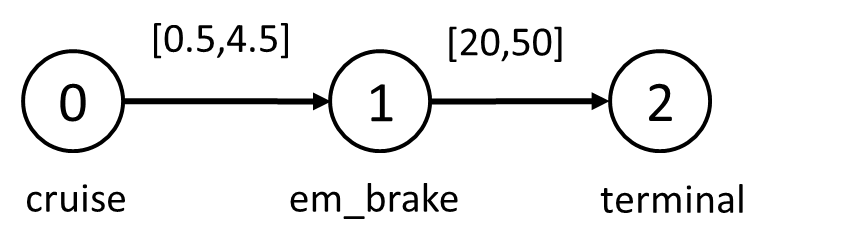
\includegraphics[width=\textwidth]{brake_2_modes.png}
        \caption{\small Transition graph $G_1$.}
        \label{fig: em_brake_graphsA}
    \end{subfigure}
    \begin{subfigure}[b]{0.3\textwidth}
        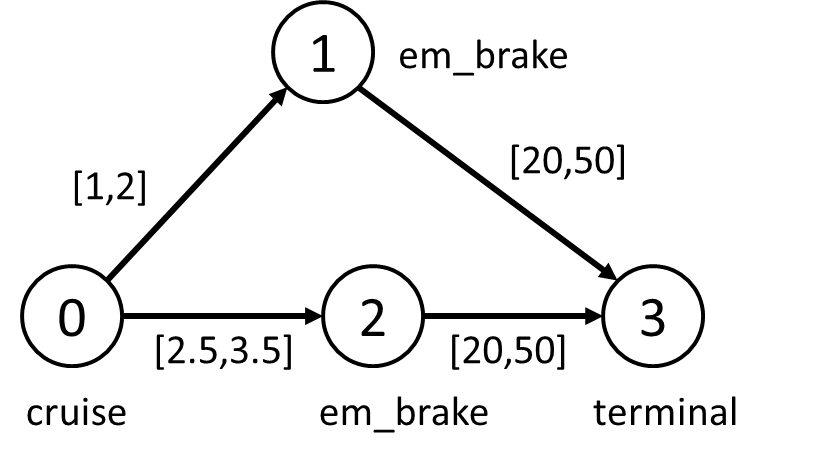
\includegraphics[width=\textwidth]{brake_3_modes.png}
        \caption{Transition graph $G_2$.}
        \label{fig: em_brake_graphsB}
    \end{subfigure}
    \begin{subfigure}[b]{0.35\textwidth}
	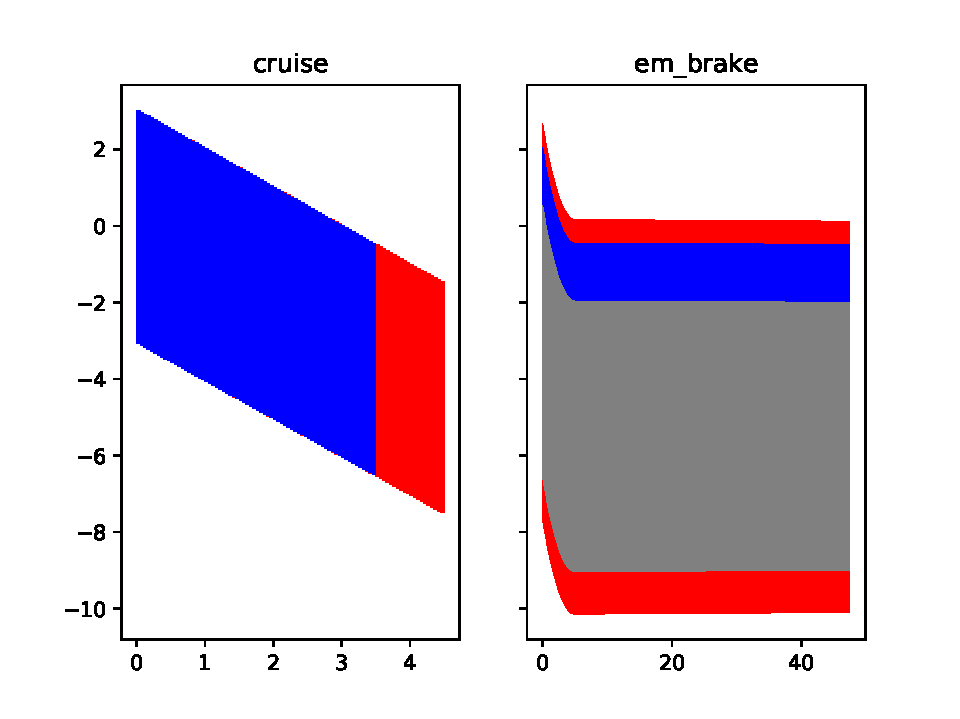
\includegraphics[width=\textwidth]{Abstraction_reachTube.pdf}
	\caption{$\auto{AEB}$ Reachtubes.}
	%\caption{Reachtubes of graphs in Figure \ref{fig: em_brake_graphs}. Red tubes corresponds to Figure \ref{fig: em_brake_graphsA}, blue and gray tubes corresonds to Figure \ref{fig: em_brake_graphsB}}
	\label{fig:abstraction}
    \end{subfigure}
\caption{\small Graphs and reachtubes for the Automatic Emergency Braking $\auto{AEB}$ system.}
\label{fig: em_brake_graphs}
\end{figure}

%
To illustrate trace containment reasoning, consider a simpler
graph $G_1$ that allows a single transition of A from \Lmode{cruise}
to \Lmode{em\_brake} over the interval bigger $[0.5, 4.5]$. Using
Proposition~\ref{prop:hybrid-contain} and checking that graph $G_2
\preceq_{\sf id} G_1$, it follows that verifying the safety of
$\auto{AEB}$ with $G_1$ is adequate to infer the safety with $G_2$.
Figure~\ref{fig:abstraction} shows that the safe reachtubes returned
by the algorithm for $G_1$ in red, indeed contain the reachtubes for
$G_2$ (in blue and gray).
%The graphs of the system, along with the reachtube plots are provided in the Appendix.
%For more complex graphs  

%Figure \ref{fig: em_brake_graphs} shows two different graphs specifying two scenarios.  
%Figure \ref{fig: em_brake_graphsA} shows that vehicle A could transit from \Lmode{cruise} to \Lmode{em\_brack} within $[0.5, 4.5]$. However, in  Figure \ref{fig: em_brake_graphsB} the transition may happen in two disjoint time intervals $[1,2],[2.5,3.5]$. 

%Since both the vehicles never change the lane, we will only consider variables along the $y$ coordinate. The initial set is $sy_A \in [-3,3], sy_B \in [14,23], vy_A = 1, vy_B =0$. The unsafe set is set to be $|sy_A-sy_B| < 2$ ($|sx_A-sx_B| < 2$ is always satisfied).

% In the \Lmode{cruise} mode, the red tube corresponds to the vertex $0$'s reachtube in Figure~\ref{fig: em_brake_graphsA} and the blue one corresponds to vertex $0$ in Figure \ref{fig: em_brake_graphsB}. Similarly, in the \Lmode{em\_brake}, the red tube corresponds to the vertex $0$'s reachtube in Figure \ref{fig: em_brake_graphsA}, the blue tube corresponds to the vertex $1$'s reachtube in Figure \ref{fig: em_brake_graphsB} and the gray tube corresponds to the vertex $2$'s reachtube in Figure \ref{fig: em_brake_graphsB}. It can be clearly seen from Figure \ref{fig:abstraction} that in both modes,  the reachtubes of Figure \ref{fig: em_brake_graphsB} is contained in the reachtube of Figure \ref{fig: em_brake_graphsA}, which is consistent with proposition \ref{prop:hybrid-contain}.


\vspace{-10pt}
\paragraph{Sequential composition}
We revisit the $\auto{Powertrn}$ example of
Section~\ref{ex:powertrain}. The initial set $\Theta$ and unsafe set
are the same as in Table \ref{table:results}.  Let $G_A$ be the graph
($v_0$,\Lmode{startup}) $\xrightarrow{[5,10]}$ ($v_1$,\Lmode{normal})
$\xrightarrow{[10,15]}$ ($v_2$,\Lmode{powerup}), and $G_B$ be the
graph ($v_0$,\Lmode{powerup}) $\xrightarrow{[5,10]}$
($v_1$,\Lmode{normal}) $\xrightarrow{[10,15]}$
($v_2$,\Lmode{powerup}).  The graph $G_1 =$ ($v_0$,\Lmode{startup})
$\xrightarrow{[5,10]}$ ($v_1$,\Lmode{normal}) $\xrightarrow{[10,15]}$
($v_2$,\Lmode{powerup}) $\xrightarrow{[5,10]}$ ($v_3$,\Lmode{normal})
$\xrightarrow{[10,15]}$ ($v_4, $\Lmode{powerup}), can be expressed as
the composition $G_1 = G_A \seqcomp G_B$. Consider the two hybrid
systems $\H_i = \langle \L, \Theta_i, G_i, \TL \rangle$, $i \in
\{A,B\}$ with $\Theta_A = \Theta$ and $\Theta_B =
\reach{\H_A}^{v_2}$. {\toolname}'s estimate of $\Theta_{B}$ had
$\lambda$ in the range from $14.68$ to $14.71$. The reachset
$\reach{\H_B}^{v_2}$ computed by {\toolname} had $\lambda$ from
$14.69$ to $14.70$. The remaining variables also were observed to
satisfy the containment condition. Therefore, $\reach{\H_B}^{v_2}
\subseteq \Theta_{B}$.  Consider the two hybrid systems $\H_i =
\langle \L, \Theta, G_i, \TL \rangle$, $i \in \{1,2\}$, where $G_1$ is
(defined above) $ G_A \seqcomp G_B$, and $G_2 = G_A \seqcomp G_B
\seqcomp G_B \seqcomp G_B$.  Using Theorem
\ref{thm:seqcomp-mainresult} it suffices to analyze $\H_1$ to verify
$\H_2$.  $\H_1$ was been proved to be safe by \toolname\ without any
refinement.  As a sanity check, we also verified the safety of $\H_2$.
%is \Lmode{normal} $\xrightarrow{[10,15]}$ \Lmode{powerup} $\xrightarrow{[5,10]}$ \Lmode{normal} $\xrightarrow{[10,15]}$ \Lmode{term} $\xrightarrow{[0,0]}$ \Lmode{powerup} $\xrightarrow{[5,10]}$ \Lmode{normal} $\xrightarrow{[10,15]}$ %\Lmode{term} $\xrightarrow{[0,0]}$ \Lmode{powerup} $\xrightarrow{[5,10]}$ \Lmode{normal} $\xrightarrow{[10,15]}$ \Lmode{term}. 
{\toolname} proved $\H_2$ safe without any refinement as well.

